\documentclass[11pt]{article}
\usepackage[margin=1.1in]{geometry}
\usepackage{amsmath,amssymb,amsthm}
\usepackage{booktabs}
\usepackage{array}
\usepackage{graphicx}
\usepackage[round]{natbib}
\usepackage{hyperref}
\hypersetup{hidelinks}
\usepackage{microtype}

\newtheorem{proposition}{Proposition}
\newtheorem{lemma}[proposition]{Lemma}
\newtheorem{corollary}[proposition]{Corollary}
\theoremstyle{remark}
\newtheorem{remark}[proposition]{Remark}

\newcommand{\E}{\mathbb{E}}
\newcommand{\I}{\mathrm{I}}
\newcommand{\given}{\,|\,}

\title{Conformal Prediction as a Transform\\ within a Grammar for Probabilistic Forecasting}
\author{Peter Cotton\\\texttt{peter.cotton@microprediction.com}}
\date{August 2026}

\begin{document}
\maketitle

\begin{abstract}
Conformal prediction is typically presented as a bundle: a base model, a scalar
residual, and a rank-calibration step carrying an average coverage guarantee. The
dangers of chasing coverage alone are just as well documented. Building an autonomous
economic prediction system forced a different arrangement on us: a grammar of
distributional transforms in which one univariate transform embodies the conformal
step but need not terminate the processing. Its peers are the classical tools of
time-series analysis, all state-conditional bijections. This resolves the
inconsistency of treating residuals unconditionally beneath a conditional base model,
and keeps the coverage certificate where wanted, though it does not propagate down
the chain. On the economic series studied, inclusion via pooling is largely harmless
in log-likelihood and slightly beneficial in CRPS.
\end{abstract}

\section{Introduction}\label{sec:intro}

In the canonical residual-pooling pattern, a forecaster fits a conditional model and
then quotes uncertainty by ranking its past errors with every state pooled. The ranking is honest on average and silent about
tonight. That tension, conditional effort upstream and unconditional treatment at the
end, is the subject of this paper.

Split conformal prediction can be written as a chain. Fit a model, take residuals, apply
the fence-post empirical map
\begin{equation}\label{eq:fencepost}
E_n(r) \;=\; \frac{1 + \#\{i \le n : R_i \le r\}}{n+1},
\end{equation}
and map the resulting rank back through the model to a prediction set
\citep{vovk2005algorithmic,lei2018distribution}. The value of \eqref{eq:fencepost} at a
new point is a conformal p-value, and the map itself is the unrandomized conformal
predictive distribution of \citet{vovk2019nonparametric}.

We call it the fence-post
transform, after the two $+1$ corrections: $n$ points cut the line into $n+1$ cells, and
the guarantee rides on the count of cells, not of points. The knot probabilities
$i/(n+1)$ are Weibull's plotting positions, the means of uniform order statistics, so the
object is classical.

The literature mostly treats this chain as a
construction to be studied whole, and its many variants, normalized, Mondrian, quantile,
distributional, and temporal
\citep{bostrom2021mondrian,romano2019conformalized,chernozhukov2021distributional,gibbs2021adaptive,auer2023hopcpt},
as separate constructions. The nearest exceptions stop one step short. Conformal
predictive systems made the map emit a distribution function. Conformal calibrators
\citep{vovk2020calibrators} apply that map to another system's output. Both compose
once, and the map is still the last word.

We propose a different organization, in
which the map's position is a variable. The fence-post transform is
one operator. The chain is one production rule in a grammar of composable transforms. The
interesting question is then not which conformal method to choose but which sequence of
transforms minimizes the forecaster's scoring rule.

Viewed this way, conformal prediction is not, in general, an alternative that puts
statistical modeling to one side, but an integrated operator in a chain, whose
finite-sample properties may well be valuable at the point where they are computed.
Those properties distinguish it from the operators it commingles with, but they do
not privilege stopping there, nor need they remove the modeling that follows. Used
carefully in this manner, it does not materially degrade predictive quality under a
proper scoring rule, at least in our experiments.

The standard conformal pattern also carries a tension the present work avoids. A
skeptic of the standard conformal prediction patterns might reasonably ask why heavy
anchoring on the empirical distribution (in a sense, not modeling at all) is
appropriate in the context of model residuals, whereas to apply the same emphasis in
general would be absurd.

The stock answer is about targets. For marginal coverage, pooling is justified by
exchangeability of the residuals alone, a weaker and testable hypothesis, and
distribution-free conditional coverage is provably out of reach
\citep{vovk2012conditional,lei2014distribution,barber2021limits}, so the pooled law
is what one settles for.

That answer is not satisfactory for a forecaster scored by a
proper scoring rule. There the pooled residual law is quoted as a predictive density,
its adequacy is exactly conditional invariance, and the certificate does not establish
that. Certifying ranks under exchangeability makes stopping at the pooled law a
modeling decision, not a consequence of the guarantee.

In univariate probabilistic forecasting, Platt scaling,
isotonic and quantile recalibration, temperature scaling, conformal predictive systems,
and distributional conformal prediction can all be represented as monotone recalibration
operators on a scalar predictive, score, or probability coordinate, differing in what
they fit and what they guarantee
(Section~\ref{sec:family}). The fence-post transform is the member with a certificate,
and the certificate is a positional type annotation on one operator inside a composable
predictive program: a reason to admit the operator to the grammar, and nothing more.

This reorganization has content because the fence-post operator composes. Once interpolated,
$E_n$ is an invertible change of variables with a density, and its probit composition
$z = \Phi^{-1}(E_n(r))$ maps exchangeable residuals to approximately standard Gaussian
coordinates. Nothing obliges a forecaster to stop there. One can fit further structure on
the Gaussianized stream, transform again, and continue, exactly as one does with any other
member of the transform library. Conformal calibration stops at the transform. The grammar
keeps going.

Two testable claims follow. The first is that the operator is not a natural stopping
point: a serial model fitted on the Gaussianized stream can beat quoting the
transformed empirical law where it stands, when exploitable residual structure
remains. The second is that nesting is
cheap: a pool over chains that includes the conformal pattern should not pay materially
for admitting it, because the pool reallocates weight away from the pattern on series
where it is a bad choice. We confirm both on a corpus of economic series and quantify a third
finding we did not anticipate: the operator's incremental value inside a fixed chain
depends on the scoring rule, and the dependence is not explained by the smoothing we
tested.

A companion paper prices what a fixed representation choice costs
\citep{cotton2026gap}. Under logarithmic loss the irreducible cost of pooling residuals in
given coordinates is a mutual information, the conformal information gap, and the companion
measures it on the same corpus. The present paper is the constructive complement. If a fixed
conformal pattern can be a bad choice with a quantifiable price, the remedy is not a better
fixed choice. It is a grammar in which the choice is made by the scoring rule, online,
per series.

\section{The fence-post transform as an operator}\label{sec:operator}

We work with online univariate transforms in the sense of the \texttt{skaters} library,
described at length in a methods paper \citep{cotton_skaters} and briefly in a software
paper \citep{cotton_skaters_joss}. A transform is a pair of functions. The forward function consumes
one observation and its own past state and emits a transformed observation. The inverse
function maps predictive distributions in the transformed space back to the original space.
Conditional on its own past state, the forward map is an invertible change of variables in
the current observation, so predictive densities push back exactly, Jacobians included.

The raw fence-post map \eqref{eq:fencepost} is a step function. It has no density and no
inverse, so it is not a transform in this sense. The minimal repair is interpolation,
minimal but not unprecedented \citep{harar2022redistributor}. Let
$y_{(1)} \le \dots \le y_{(n)}$ be the past observations, place knots at the order
statistics with fence-post probabilities $p_{(i)} = i/(n+1)$ for
$i = 1, \dots, n$, set
$z_{(i)} = \Phi^{-1}(p_{(i)})$, and interpolate the pairs $(y_{(i)}, z_{(i)})$ piecewise
linearly. We call the resulting operator \emph{gaussianize}. The knot values are the
left limits of the right-continuous map \eqref{eq:fencepost} at the calibration points,
and this convention is what makes the certificate exact at the knots
(Proposition~\ref{prop:grid}). That is the full map. The implementation retains at
most $39$ of the knots, chosen at equal mass from the full sorted history so that
each retained knot is an exact order statistic until the slope guard below binds, and
drops any knot whose value ties its neighbor, so ties widen the retained cells. We write gaussianize-full for the map
through every knot and gaussianize for the implemented retained-knot member.
Proposition~\ref{prop:sparse} prices the difference: the certificate is a function of
the retained resolution.

The interpolation changes
the object, and Section~\ref{sec:typing} states exactly what survives the change: the
discrete map's output is a function of ranks alone, while the interpolated map's output
depends on spacings as well, so the two are different operators with different
certificates.

Beyond the edge knots the map
extends linearly in $(y, z)$ coordinates, and linearity in the probit coordinate is a
Gaussian tail in the observable, with scale set by the spacing of the extreme quantiles.
Tail mass is unobservable, so any usable version of the operator carries a tail assumption,
and this is the mildest one consistent with the coordinates. A kernel-smoothed variant
replaces the empirical distribution function with a Gaussian-kernel estimate at Silverman
bandwidth, represented by a monotone $C^1$ cubic through the same knots, and we use it in
Section~\ref{sec:smooth} to test whether smoothness matters.

Two guards complete the definition, and both were forced by data rather than taste. First,
every knot segment's inverse slope $dy/dz$ is capped at twenty times the
interquartile inverse slope, so the forward slope is bounded below. An upstream
variance collapse can plant a many-sigma outlier as an edge knot, and an uncapped edge
segment then hands the inverse map an explosive extrapolation slope. The cap is an explicit
assumption: tail scale at most a fixed multiple of the central scale.

Second, the value handed downstream is clamped to $|z| \le 8$. The clamp applies
only to the coordinate supplied to downstream state updates and is not part of the
invertible map used to construct or pull back predictive densities, so the
change-of-variables identity is intact. When it binds, the downstream learner is updated
with a bounded surrogate rather than the literal transformed observation, and that
alteration can persist through the learner's state. In the type system the two objects
are distinct: gaussianize is invertible and density-carrying, and the bounded update
channel is a winsorized learner input, not a transform.

Within the knot range the clamp cannot bind, since no
fence-post rank exceeds probability $n/(n+1)$ and $\Phi^{-1}(n/(n+1)) < 8$ for any
feasible $n$. It can bind on the extended tail and on degenerate warmup emissions, and
the latter is why it exists, because downstream learners have expanding memory. In one series in our corpus a degenerate warmup emitted a single
transformed value near $8000$, and the downstream Welford variance and recursive
least-squares state never forgot it, inflating that series' loss by four orders of
magnitude. Composability is not free. An operator that is harmless as a terminal step can
poison downstream learners through one bad emission, and the operator's definition has to
prevent this, not the caller.

The guards are better read as declared budgets than as patches. Invertibility alone is
too weak a property for a chain. The pullback quantile $y_\alpha = m^{-1}(q(\alpha))$
inherits the steepness of the inverse map $m^{-1}$, and beyond the edge knots the inverse
is an assumption rather than an estimate, because tail mass is unobservable at any $n$.
The slope cap makes the assumption finite. It declares that $m^{-1}$ is Lipschitz, with
constant $L$ equal to twenty times the central inverse slope, and the declaration buys a
guarantee. The declaration also has a price: a binding cap moves knots off their
order statistics, and Appendix~\ref{app:certificate} prices the displacement.

\begin{lemma}[Pullback quantiles are budgeted]\label{lem:budget}
Let $m$ be a strictly increasing forward map whose inverse is $L$-Lipschitz on all of $\mathbb{R}$,
extrapolation included, and let $q$ be the quantile function of the predictive in
transformed coordinates. Then the pulled-back predictive has quantiles
$y_\alpha = m^{-1}(q(\alpha))$ and
\[
  |y_\alpha - y_{1/2}| \;\le\; L\,\big|q(\alpha) - q(\tfrac12)\big|
  \qquad \text{for every } \alpha \in (0,1).
\]
For a chain of such maps the same bound holds with $L$ the product of the rungs'
constants.
\end{lemma}

\begin{proof}
Monotone maps transport quantiles, so $y_\alpha = m^{-1}(q(\alpha))$. The Lipschitz bound
applied to the pair $q(\alpha), q(\tfrac12)$ gives the display. A composition of
Lipschitz maps is Lipschitz with the product constant.
\end{proof}

With a Gaussian leaf of scale $\sigma$ the right side is
$L\sigma\,|\Phi^{-1}(\alpha)|$. The budget is conditional on the operator's state:
$L$ is twenty times the current central inverse slope and $\sigma$ is fitted, so the
lemma bounds quoted quantiles relative to the current central scale, not by a
universal constant. Within that reading, no realization amplifies a quoted quantile
past its budget. The global $L$ is also purchased with the knot displacement of
Remark~\ref{rem:guard}: the Lipschitz budget and retained-level exactness are
competing constraints, and no operator holds both exactly on arbitrary data. The naive empirical map declares $L = \infty$ and buys nothing. The clamp is
the same discipline in the forward direction. The retained knot coordinates lie
within $(-8, 8)$ for every practical history length, so the clamp controls only
extrapolated and warmup emissions, and a downstream learner with expanding memory is
safe against exactly the emissions it excludes. Any finite multiplier yields the
lemma, so the value twenty is the one remaining choice of taste, a tail-conservatism
dial. Fitting the tail where the sample reaches, generalized-Pareto by censored maximum
likelihood as the leaf already does, with the budget kept as a prior bound, is the
refinement we leave open \citep[the tail instability of the normal quantile
transform is documented by][]{bogner2012normal}.

Before enough observations accumulate, the operator standardizes by expanding moments,
which is the $n \to 0$ limit of the empirical map. After the warmup the knots are rebuilt each step, at most
thirty-nine of them at equal mass from the full sorted history, so the retained knots
sit at exact order statistics, and carry no rank-approximation error while the slope
guard is inactive. The sorted buffer
itself grows with the series. A bounded compacted sketch is the obvious refinement, and
its price is the rank-error term of Proposition~\ref{prop:sparse}.

\section{What composition preserves}\label{sec:typing}

A \emph{chain} is a finite word
$C = (T_1, \dots, T_m, L)$, stateful transforms followed by a terminal leaf. A
transform is a tuple: a forward emission, an inverse pullback, a state update, a clock,
input and output types, and declared properties. The forward map consumes an
observation and the operator's state and emits a coordinate. The pullback carries
predictive laws backward. The clock says when the state may absorb data. The properties
are judgments, monotone, invertible, density-carrying, inverse-Lipschitz with a
declared budget, exchangeability-preserving, previsible, or $\delta$-calibrated at a position.

Composition obeys checkable rules. Invertible composed with invertible is invertible,
and Lipschitz budgets multiply (Lemma~\ref{lem:budget}). A fixed strictly increasing link
transports the grid certificate, with its levels transported along the link, because
ranks are invariant under it.
Previsible composed with previsible is previsible, since the composite map at time $t$
is built from maps measurable before $t$. A calibration certificate is not, in
general, inherited through a fitted state-dependent operator, which is the second fact
below. A pool over chains is itself an operator on chains, and
Proposition~\ref{prop:nesting} is its admission rule.

Composition preserves some properties and destroys others, and the pattern is
positional. We record the four facts that organize our experiments.

\begin{proposition}[Fence-post uniformity]\label{prop:uniform}
Let $R_1, \dots, R_{n+1}$ be exchangeable and almost surely distinct. Then
$E_n(R_{n+1})$ is uniform on the grid $\{k/(n+1) : k = 1, \dots, n+1\}$. In
particular, $\Pr\{E_n(R_{n+1}) \le k/(n+1)\} = k/(n+1)$ for
$k = 1, \dots, n+1$.
\end{proposition}

\begin{proof}
By exchangeability every ordering of $R_1, \dots, R_{n+1}$ is equally likely, and by
almost-sure distinctness the rank of $R_{n+1}$ among the $n+1$ values is uniform on
$\{1, \dots, n+1\}$. The map \eqref{eq:fencepost} evaluated at $R_{n+1}$ equals the rank
divided by $n+1$.
\end{proof}

This is the standard conformal fact \citep{vovk2005algorithmic} stated as a property of the
operator's output. It certifies the discrete map \eqref{eq:fencepost}, and the discrete
map is what the experiments do not run. The interpolated operator of
Section~\ref{sec:operator} uses spacings as well as ranks, and its output between knots
is not distribution-free. What survives interpolation is the grid, and the
accounting is mechanical. Call an operator $\delta$-conformal if, on exchangeable
almost surely distinct input, its probability-scale output is within $\delta$ of
calibrated at every level. Any interpolation through every knot is
$1/(n+1)$-conformal, exact at the knots. The implemented $39$-knot map is conformal
to roughly one part in forty, exact at its retained levels while its guard sleeps.
Compression, a binding guard, and ties each pay a price.
Appendix~\ref{app:certificate} states and proves the prices, a leave-one-out
version for data-dependent guards among them, and a counterexample where the moving
cap dominates. The certificate is priced in the operator's computational budget, and
none of the prices moved the campaign's scores.

What separates them is the exact statement. The discrete map is deterministic,
exactly calibrated at every grid level, noninvertible, and $1/(n+1)$-calibrated between
grid levels. Randomized smoothing, which spreads each output uniformly over its rank
cell, is exactly calibrated at every level and is a stochastic kernel rather than a
deterministic transform \citep{vovk2005algorithmic}. The interpolated map is
deterministic and invertible, stays exact on the grid, and incurs at most one full-grid
cell of calibration error elsewhere. The grammar uses the deterministic, invertible version and quantifies its one-cell calibration relaxation.

The exact conformal object is a rank certificate, and a rank certificate is not a
predictive density. Turning it into one requires interpolation, smoothing, tail
assumptions, and model selection, the same choices met everywhere else in probabilistic
forecasting, and exchangeability supplies none of them.

The log score will still notice: it
integrates the predictive density between grid points and in the tails, exactly where
the certificate is $\delta$-relaxed and assumption-laden, and
Section~\ref{sec:smooth} measures what that costs.

The second fact is that this guarantee is positional. Proposition~\ref{prop:uniform}
concerns the operator's immediate output. If a downstream model is fitted on
$z_1, \dots, z_t$ and its parameters enter later forecasts, the composed system's
forecast at time $t+1$ depends on the ordering of the past stream. The exchangeability
that delivered uniformity no longer applies to the composed output. The calibration certificate
attaches to a position in the chain, not to the chain. This is not a defect. It is the
familiar price of fitting, and the reason the companion paper's ledger separates
representation, model-form, and estimation cost \citep{cotton2026gap}. But it means the
grammar has a typing discipline: an operator's guarantee names the position at which it
holds, and claims about the composed system need their own arguments.

The third fact concerns schedules, and it explains what the conformal literature's data
splitting is for and how an online chain does without it. Call a chain \emph{previsible}
if the map applied to each observation is measurable with respect to information strictly
prior to that observation. Dual use, the defect the splitting exists to avoid, is exactly
a previsibility violation: an observation flowing through a map whose state already
contains it.

Split conformal enforces previsibility with a coarse clock. Interior
operators learn on a fitting block and freeze, the terminal fence-post learns on a
disjoint calibration block and freezes, and test points meet only frozen maps.

The chains
of this paper enforce the same rule with the finest clock. Every operator emits before it
absorbs, so the map applied at time $t$ is built from $y_1, \dots, y_{t-1}$ alone, and
the past is a calibration set that never contains the present. Emit-before-absorb
enforces non-anticipation, and nothing else. It does not preserve calibration-test
exchangeability under adaptive upstream transforms, and the narrowing after
Proposition~\ref{prop:sequential} makes the difference from splitting precise.

On the exchangeable hypothesis the fine clock matches the batch guarantee and adds
independence across time.

\begin{proposition}[Sequential fence-post outputs are independent]\label{prop:sequential}
Let $Y_1, \dots, Y_T$ be exchangeable and almost surely distinct, and let
$U_t = E_{t-1}(Y_t)$ be the fence-post transform of $Y_t$ through the map built from
$Y_1, \dots, Y_{t-1}$, as in \eqref{eq:fencepost} with $n = t - 1$. Then
$U_1, \dots, U_T$ are independent, and $U_t$ is uniform on $\{1/t, \dots, t/t\}$.
\end{proposition}

\begin{proof}
Let $K_t \in \{1, \dots, t\}$ be the rank of $Y_t$ among $Y_1, \dots, Y_t$. From
\eqref{eq:fencepost} with $n = t-1$,
$U_t = \big(1 + \#\{i < t : Y_i \le Y_t\}\big)/t = K_t / t$. The full ranking of
$Y_1, \dots, Y_T$ is a permutation $\pi$ of $\{1, \dots, T\}$, and the map
$\pi \mapsto (K_1, \dots, K_T)$ is a bijection onto
$\{1\} \times \{1,2\} \times \dots \times \{1, \dots, T\}$: given the sequential ranks,
the permutation is reconstructed by inserting each element at its stated position, and
both sets have cardinality $T!$. Exchangeability with almost-sure distinctness makes
$\pi$ uniform over the $T!$ orderings, so $(K_1, \dots, K_T)$ is uniform over the product
set. Uniformity over a product set is independence of the coordinates, each uniform on
its factor.
\end{proof}

The independence of sequential ranks is classical \citep{renyi1962} and powers online
exchangeability testing \citep{vovk2003testing}. The proposition concerns the discrete
sequential ranks alone. The interpolated coordinates carry spacing information, and no
independence is claimed for them.

Previsibility is not a substitute for splitting. It prevents leakage, the map at
time $t$ not containing $y_t$, and that is all it prevents. It does not make the transformed stream exchangeable: previsible
strictly increasing maps that differ across time destroy exchangeability trivially,
as when every second observation is shifted by a constant. Splitting does more. It
freezes one map for calibration and test, so their scores stay exchangeable whenever
the data are. The accurate statement is that emit-before-absorb guarantees prequential
out-of-sample evaluation, and if the stream arriving at the fence-post rung is itself
exchangeable, its sequential ranks are independent. The chains of
Section~\ref{sec:experiments} do not satisfy that hypothesis, and their certificate
reads through the idealization already declared. Here the proposition separates the
schedules. Split
conformal's p-values share one calibration set and are dependent. The prequential
outputs are independent, and the price is early resolution: the map at time $t$ has
granularity $1/t$, hence the warmup of Section~\ref{sec:operator}.

The certificate survives any further fixed monotone map, the probit included, because
monotone maps preserve ranks. It is not automatically inherited through a downstream
fit, by the second fact,
and a chain that wants a terminal certificate ends with one more fence-post step on the
final residuals. Full conformal is a third schedule, symmetrizing the whole chain over
the data at the cost of refitting per candidate value \citep{vovk2005algorithmic}. We do
not use it. An operator's annotation is therefore a position and a clock.

For the economic series of Section~\ref{sec:experiments} the exchangeable hypothesis of
Proposition~\ref{prop:sequential} is false, as it is throughout time-series conformal
prediction, so the uniformity claims are conditional on model adequacy. Previsibility is
not. It holds by construction, and every score in this paper is out-of-sample even where
the guarantee hypothesis fails. The contracts so far assemble into the beginning of the
type table the conclusion asks for:

\begin{center}
\footnotesize
\setlength{\tabcolsep}{4pt}
\begin{tabular}{lllp{5.2em}>{\raggedright\arraybackslash}p{11em}}
\toprule
operator & previsible & exch.-preserving & invertible & certificate \\
\midrule
fence-post, discrete & yes & indep.\ seq.\ ranks & no &
  exact at grid levels \\
gaussianize, full grid & yes & not claimed & yes &
  exact on all $n$ rank levels, $1/(n{+}1)$ globally \\
gaussianize, implemented & yes & not claimed & yes &
  exact on retained levels (distinct input, guard inactive), $\Delta_n$ plus guard
  displacement \\
fixed monotone link & yes & yes & yes & transparent \\
EMA location, EWMA scale & yes & no & given state & none \\
frozen split-fitted model & yes, coarse clock & cal/test pairs & varies & none \\
refit on the stream & yes & no & given state & none, blocks pass-through \\
\bottomrule
\end{tabular}
\end{center}

The middle column is the working hypothesis of every chain in
Section~\ref{sec:experiments}: location and scale do not preserve exchangeability, so the
fence-post rung downstream of them operates under an idealization, which the contracts
state rather than hide.

The fourth fact prices the choice of coordinates. The companion paper's transform-pooling
theorem states that pooling residuals $R$ after an invertible state-dependent change of
coordinates $\phi_X$ has irreducible log-score gap $\I(\phi_X(R); X)$, the mutual
information between the transformed residual and the state $X$ on which its true
conditional law depends: the Jacobians of the
transform cancel, and only the coordinates' ability to remove conditional heterogeneity
matters \citep{cotton2026gap}. The gaussianize operator is a data-dependent monotone map,
measurable with respect to its own past state, and piecewise $C^1$, so conditional on the
state the theorem's hypotheses hold. The grammar view adds only this: since operators
compose, the coordinates in which one pools are themselves a product of the chain, and the
gap is a property of the whole chain up to the pooling point.

The operator's ancestry is long. The
branches are not one idea. They transform different objects for different reasons, and
what they share is the trunk: push an observation through a distribution function and
work on the flat scale.

The
empirical distribution function is Galton's ogive \citep{galton1875}. Plotting positions
place ordered observations at chosen probabilities, from Hazen's $(i - \tfrac12)/n$
onward \citep{hazen1914}, with $i/(n+1)$ being Weibull's position
\citep{weibull1939}, and
the probability integral transformation received its name and first systematic treatment
from \citet{pearson1938}. Normal scores, the replacement of ranks by standard-normal
quantiles, are the gaussianize map's direct ancestor \citep{vanderwaerden1952}. That
estimation spoils the transform's exactness has been known since
\citet{davidjohnson1948}, and the positional fact above is its descendant.

Rosenblatt's
chaining through conditional distributions whitens any process
\citep{rosenblatt1952remarks}, and normalizing flows are its learned, offline
descendants \citep{tabak2010,papamakarios2021normalizing}. Parametric monotone
Gaussianizers run from \citet{boxcox1964} to \citet{yeojohnson2000}. Quantile
mapping in the geosciences is the same move under another name
\citep{panofskybrier1968}. Transformed residuals as model criticism begin with
\citet{coxsnell1968}, and the PIT as a forecast-evaluation instrument with
\citet{diebold1998evaluating}. The prequential stance that all of this paper's
scoring obeys is \citet{dawid1984present}.\footnote{A fuller annotated timeline is maintained at
\url{https://skaters.microprediction.org/heritage.html}.}

Modeling after marginal Gaussianization is classical outside conformal prediction
too. \citet{chenfan2006} estimate an unknown time-series marginal by the rescaled
empirical distribution with denominator $n + 1$, model temporal dependence with a
parametric copula on the probability scale, and invert the fitted transition law for
conditional forecasts. Meta-Gaussian hydrologic processors place the normal quantile
transform inside a Gaussian predictive model and map back \citep{bogner2012normal}.
Autoregressive transformation models write the conditional law as a monotone
transformation of a fixed base distribution \citep{rugamer2023autoregressive}. The
distinction here is not the transform, model, inverse architecture. It is the
finite-sample grid certificate attached to the empirical operator, the regularity
debit charged against it, the online clock and state semantics, and score-based
pooling over composed chains.

The transform also ran as a market before it ran here as an operator. The
microprediction platform's z-streams solicited competitive real-time predictions of
PIT-transformed residual streams \citep{cotton2022microprediction}, chaining
solicitations so that one crowd predicted the residuals of another's forecasts. That is
interior composition as a mechanism, and the algebra of such mechanisms is developed in
\citet{cotton2026algebra} and \citet{cotton2026multistage}. The grammar of this paper
is the single-forecaster form of the same design.

Against this ancestry the
fence-post operator's distinction is narrow and real: at its position, on exchangeable
input, its ranks carry a finite-sample certificate.

\section{Measurements}\label{sec:experiments}

\subsection{Design}\label{sec:design}

The corpus, scoring conventions, and evaluation protocol follow the companion paper
\citep{cotton2026gap}. We use 701 FRED change series with at least 600 observations and
repeat fraction below five percent. The series are latest-vintage changes, so the claims
concern sequential modeling of economic-shaped sequences, not operational real-time
forecasting, where revisions and publication lags would enter. Every forecaster runs prequentially: at each time it
issues a one-step predictive density from data strictly before that time, then sees the
observation and updates. Scoring starts after a burn-in of 300 observations. The predictive in the original coordinates is the finite Gaussian mixture produced by
the nine-particle inverse. That implemented mixture, blended with weight $0.01$ toward
an expanding-window Gaussian reference, is scored exactly, with no clipping or
flooring in the reported nats. CRPS is computed in closed
form from the Gaussian-mixture predictive. Per-series CRPS is normalized by the location
baseline defined next, so scales are comparable across series.

The bare leaf, six single chains, and three pools are compared. All chains end in a Gaussian leaf with
online variance, and all transforms update online.

\begin{center}
\small
\begin{tabular}{ll}
\toprule
config & chain \\
\midrule
A & location (EMA) $\to$ leaf \\
B & location $\to$ scale (EWMA standardize) $\to$ leaf \\
C & location $\to$ gaussianize $\to$ leaf \quad (rank-transform chain) \\
D & location $\to$ scale $\to$ gaussianize $\to$ leaf \quad (normalized rank-transform chain) \\
E & location $\to$ scale $\to$ gaussianize $\to$ AR(1) $\to$ leaf \quad (refit through) \\
F & location $\to$ scale $\to$ AR(1) $\to$ leaf \quad (same refit, no gaussianize) \\
G & likelihood-weighted pool over $\{$leaf, A, B, C, D, E, F$\}$ \\
H & likelihood-weighted pool over $\{$leaf, A, B, F$\}$ \quad (G minus the gaussianize chains) \\
I & the pool of G with kernel-smoothed gaussianize \\
\bottomrule
\end{tabular}
\end{center}

Configs C and D are the conformal production rule written as a chain: transform, apply the
fence-post empirical map, stop, and read the predictive off the inverse. Config E continues
through the operator. The pools use the same likelihood-weighted online ensembling as the
companion paper's forecaster, with a complexity penalty by chain depth.

A second campaign, run for this revision, adds the decomposition ladder and robustness
grids reported below. Config D0 is config D with its fitted leaf replaced by the fixed $N(0,1)$ law, the
literal conformal terminal forecast, and a full-grid variant retains every knot. Alternative fixed links replace gaussianize in the E position. Guard and
resolution grids, an iid null suite, and a CRPS-weighted pool complete the set. The
refetch recovers $572$ of the $701$ series, mostly dropping short monthly ones, and
the campaign runs use those, with percentile bootstrap intervals resampling series.
The dropped series carried more of the operator's log-score tax on the original
run. That is part of why the tax reads $0.079$ nats here against $0.108$ there, and
the rest is data vintage. The corpus can always grow.
Figure~\ref{fig:duels} summarizes the comparisons behind the paper's three findings.

\begin{figure}[t]
\centering
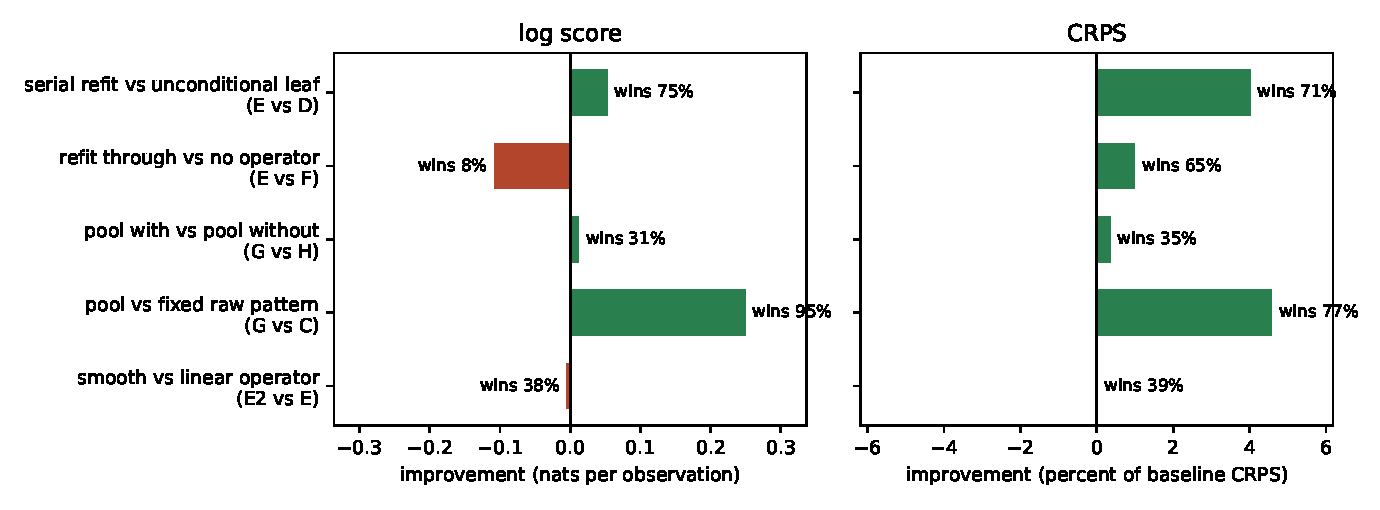
\includegraphics[width=\textwidth]{fig_grammar.pdf}
\caption{The five comparisons behind the three findings, under both scoring rules,
with each duel's corpus in its label. Bars to the right favor the first-named config.
Log score improvement is in nats per observation. CRPS improvement is the mean
per-series ratio, expressed as the percent cut. Win rates are per-series.}\label{fig:duels}
\end{figure}

\subsection{Stopping and inserting are different questions}\label{sec:interior}

In conformal practice the empirical map is terminal. One fits a model, ranks the
residuals, and quotes the ranked law as the predictive. The fence-post step is where
inference ends, and the design assumes the residuals arrive exchangeable, with nothing
left in them worth modeling. Config D is that pattern written as a chain up to one caveat: its terminal leaf is a
fitted unconditional Gaussian. Config D0 removes the caveat by quoting the fixed
$N(0,1)$ law at the operator's output, which is the literal conformal terminal
forecast. Config E reads
the same operator differently: its output is a coordinate system, and whatever structure
the model missed is easier to fit in those coordinates. The two readings are testable
against each other. For the exact sequential ranks, exchangeable input leaves no serial
rank signal for a refit to find, by Proposition~\ref{prop:sequential}. The interpolated
coordinates carry spacing information besides, and an estimated AR(1) brings estimation
noise of its own, so the comparison is informative rather than clean.

The ladder, on the $572$-series campaign corpus, separates three prices. Knot compression is free: the full-grid variant
differs from $39$-knot D0 by $0.003$ nats, compressed ahead. Refitting the terminal
leaf hurts: D scores $0.027$ nats below D0 and wins $3$ percent of series, because the
operator has already standardized its output and a fitted variance adds estimation
noise. Serial refitting beats the literal stop on average: E improves on D0 by $0.019$
nats (interval $0.011$ to $0.029$) and cuts the mean per-series CRPS ratio by $3.9$
percent, winning $66$ percent of series on CRPS. The mean CRPS gain is tail-driven,
with a median cut of $0.3$ percent, and the log-score wins are a minority. E beats D0
on a third of series, loses slightly on the rest, and gains a lot where it gains.
Against the fitted-leaf D the margin is $0.046$ nats with $73$ percent wins.

Under the log score the oracle version of this
margin is the predictive mutual information remaining in the transformed stream, the
quantity the companion paper's ledger prices \citep{cotton2026gap}. The measured margin
is the part of it an AR(1) captures, net of estimation cost. Serial structure survives
the transform, and exploiting it is a skewed trade rather than a uniform one: the
conformal stopping point is defensible series by series and beaten on the corpus.

A synthetic experiment shows the mechanism in isolation. Let $z_t = 0.8 z_{t-1} +
\varepsilon_t$ and observe $y_t = \mathrm{sign}(z_t) |z_t|^{1.5}$, a monotone warp of an
AR(1), which obscures the linear representation without removing the dependence. Stopping at
gaussianize scores $-1.56$ nats and $0.62$ CRPS. Refitting AR(1) through it scores $-1.07$
and $0.41$, beating both the stop and the same AR chain without the operator ($-1.16$,
$0.42$). When the downstream learner is well specified only in the empirical map's
coordinates, passing through the operator beats both stopping and applying the same
learner in the original coordinates.

Stopping is one question, and inserting is another. E versus D0 asks whether the
rank transform is a good architectural stopping rule. On average the answer is no. On
most individual series it is yes. The
operator's incremental value is E versus F, the same refit without the operator, and
that answer is score-dependent. Under CRPS
the operator helps: E beats F on $64$ percent of series and holds the best CRPS in the
study. Under the log score the operator costs $0.079$ nats against F on the campaign
corpus and wins $9$ percent of series. We return to this in
Section~\ref{sec:smooth}, because the natural suspicion, that the piecewise-linear density
is to blame, turns out to be wrong.

The alternative links sharpen the point. A fixed Cauchy link in the same position, the
probit of the standard Cauchy distribution function, costs $0.007$ nats against F on
the mean, with an interval spanning zero. Series by series it loses to F seventy
percent of the time, by small margins. It captures about half of the operator's mean
CRPS gain. A sinh-arcsinh link with $\delta = 0.5$ pays no
material tax either and wins the per-series CRPS comparison against the operator on
$61$ percent of series, though not on average. The rank map keeps the best mean CRPS,
beating the Cauchy link on $72$ percent of series, and pays for it in nats. Much of the
operator's architectural value is heavy-tailed monotone reshaping that a fixed smooth
link supplies without a tax. What the fixed link cannot supply is the certificate.

\subsection{Nesting limits the cost of admission}\label{sec:nesting}

The raw conformal pattern C is a reasonable forecaster on this corpus, better than the
location baseline on average under both scores. It is also, on a minority of series, a bad
choice. Config G, the likelihood-weighted pool over all seven chains, gaussianize chains
included, beats the fixed pattern C on $95$ percent of series by log score, by $0.249$
nats on average. On the twenty series where C is worst, with relative CRPS $1.020$, the
pool sits at $0.843$ on the same series. The pool walks away from the production rule
where it underperforms.

Admitting the pattern is approximately free on average. The average hides the shape. Config H, the same pool with the gaussianize chains removed, differs
from config G by $0.012$ nats and $0.4$ percent of baseline CRPS, with the nesting pool
G ahead on both means. Per series the picture is lopsided. G wins under a third of series by log score and
just over a third by CRPS, and its median difference from H is zero to four decimals.
Its fifth-percentile loss is under a thousandth of a nat, and its ninety-fifth-percentile
gain is twenty times larger. Frequent negligible losses buy occasional real gains. Under
the log score this shape is not luck. A standard Bayes-mixture regret inequality
applies, and its interest here is what the subset represents: the conformal chains as a
candidate block whose admission has a price.

\begin{proposition}[Nesting is cheap under the log score]\label{prop:nesting}
Let the pool predictive be the Bayes mixture over chains with prior $\pi$, and let
$q_t$ be the predictive of the renormalized sub-mixture over any subset $Q$ of chains,
with prior mass $\pi_Q$. Then for every realization $y_1, \dots, y_T$,
\[
  -\sum_{t=1}^T \log p_t(y_t) \;\le\; -\sum_{t=1}^T \log q_t(y_t)
  \;+\; \log\frac{1}{\pi_Q}.
\]
\end{proposition}

\begin{proof}
For a Bayes mixture the cumulative predictive likelihood telescopes to the prior-weighted
sum of the chains' likelihoods,
$\prod_t p_t(y_t) = \sum_c \pi_c \prod_t p_{t,c}(y_t)$. Dropping the chains outside $Q$
and renormalizing,
$\prod_t p_t(y_t) \ge \pi_Q \sum_{c \in Q} (\pi_c/\pi_Q) \prod_t p_{t,c}(y_t)
= \pi_Q \prod_t q_t(y_t)$. Take logarithms.
\end{proof}

Take $Q$ to be the sub-pool without the gaussianize chains. The total price of
admitting them is then at most $\log(1/\pi_Q)$ nats, however the data falls, and the
per-observation price vanishes. The mass $\pi_Q$ is the prior mass of the retained
block, not of the admitted one. The proposition applies
to the untempered Bayes pool with the depth prior applied once. The implemented pool
tempers the likelihood update at rate $0.8$ and applies its depth penalty per step, for
adaptivity under regime change, so the measured G-versus-H comparison is empirical and
does not inherit the exact bound.

Rerunning both pools as genuine Bayes mixtures reproduces the comparison on a fresh
data vintage. There is no likelihood clipping and no cross-expert mixture pruning, the reference
blend sits inside the weight updates, and the depth prior is applied once, so the
telescoping identity applies verbatim to these scores. The operator's $|z| \le 8$
learner-input channel stays active inside each expert, as everywhere in the paper. G is ahead of H by $0.012$ nats on average over
$572$ series, with the same lopsided shape, wins on one series in ten, and median
difference zero. The sub-pool prior mass is $\pi_Q = 0.573$, so the proposition's
worst case is $0.56$ nats in total however long the series run. The realized
comparison sits on the profitable side of it. Nothing
in the reported comparison hinges on the tempering. The measured $0.012$
nats in G's favor says this corpus more than repays the admission.

No such bound is available to us
under CRPS, and there the claim stays empirical. The
weights update by likelihood, so the log score does the choosing and CRPS only evaluates
the chosen blend. The matching experiment is a CRPS-weighted exponential pool over the
same seven chains with the same prior. It beats the exact Bayes pool under the log
score, by $0.021$ nats per observation with wins on $76$ percent of series. The CRPS
comparison is mixed. It wins $64$ percent of series with median ratio $0.99$, and it
loses on the mean ratio, $1.003$, because a few series blow out. The admission rule
is itself a choice within the grammar, and likelihood weighting is not obviously the
right one. Why the log-score-driven chooser loses in its own metric is an open
question we flag rather than resolve.

This is the practical content of the grammar view. A fixed conformal method is
a commitment, and the companion paper prices what the commitment can cost. A grammar that
contains the method as one rule converts the commitment into a weighted vote, and the vote
is revised online by the scoring rule. Nesting does not avert disasters on this corpus,
because the guarded operator does not produce disasters. An exact Bayes pool trims the bad tail at a bounded cumulative price, vanishing per
observation. The tempered pool used here exhibits the same behavior empirically.

\subsection{The tested smoothing does not remove the tax}\label{sec:smooth}

The log-score cost of the operator invites an implementation explanation: the
piecewise-linear empirical map has a piecewise-constant density, and the log score punishes
kinks. The kernel-smoothed $C^1$ variant tests this directly, replacing the interpolated
empirical distribution function with a smooth kernel estimate while changing nothing else.
The smooth variant tracks the linear one within $0.012$ nats and $0.2$ percent of
baseline CRPS in every position, and against config F it costs $0.113$ nats where the
linear variant cost $0.108$. Both numbers are from the original $701$-series run,
whose tax exceeds the campaign corpus's $0.079$ for the composition and vintage
reasons of Section~\ref{sec:design}. The tested smoothing does not explain or remove
the tax.
Alternative bandwidths, adaptive tails, and splines tuned under log loss remain
untested, and the remaining evidence points at resolution and tail specification.

The tax is not the kinks, and it is the same structure the companion paper measured for
terminal empirical pooling. An empirical map's resolution is bounded by its ranks, and its
tails are an assumption, and the log score is exactly the score that pays for resolution
and tails. Under CRPS, which pays for calibrated quantiles, the operator earns its place in
the chain. Under the log score a fitted parametric leaf on the same stream is worth more.
The value of the fence-post operator, like the value of residual pooling in the companion
paper, depends jointly on the coordinates, the estimator, and the scoring rule. The grammar
does not remove this dependence. It locates it: the scoring rule chooses among chains, and
the operator is a candidate, not a default.

The probit is likewise a choice, not the point. Composing the operator with any further
fixed invertible link leaves the representation content unchanged, since mutual information
is invariant under invertible maps, so the transform-pooling theorem makes the link
representation-irrelevant. What remains is model form. On a 120-series holdout check, a
logistic link in place of the probit shifts results by hundredths of a nat under both
scores, and the shift consistently favors the logistic: the Gaussian leaf pushed through
the heavier-tailed link implies a heavier-tailed predictive, which fits real standardized
residuals slightly better. The theorem fixes only the representation content. A link can still matter to a
restricted downstream learner through specification and estimation, and on this corpus
it acts as a small tail-shape choice, an empirical observation rather than a
consequence of the theorem.

\subsection{Robustness}\label{sec:robust}

Three checks bound the sensitivity of these findings. An iid null suite measures how much serial signal the adaptive interpolation
invents when there is nothing to find. The kinds are Gaussian, Student $t_3$,
lognormal skew, and a two-component mixture, forty replicates each. The largest E
minus D log-score delta across kinds is $0.0013$ nats, with standard error of the
same size, against a headline effect sixteen standard errors larger.
A guard grid crossing slope caps $\{10, 20, 40\}$ with clamps
$z_{\max} \in \{6, 8, 10\}$ on a hundred-series subsample moves config E by
$0.0013$ nats end to end, so the guard constants are not doing the work. A resolution
grid on the same subsample finds the knot count flat in the point estimates: $79$,
$159$, and the full grid all sit within $0.003$ nats of $39$, with intervals spanning
zero. On a hundred series those intervals cannot exclude effects of the size the
particle count shows. Raising the inverse from nine particles to nineteen is worth
$0.015$ nats, and going further is not. The certificate's resolution parameter is not the empirical bottleneck. The
inverse's resolution is, mildly.

\section{One family}\label{sec:family}

The grammar view collapses a scattered vocabulary. Platt scaling
\citep{platt1999probabilistic}, isotonic calibration \citep{zadrozny2002transforming},
temperature scaling \citep{guo2017calibration}, quantile recalibration
\citep{kuleshov2018accurate}, conformal predictive systems \citep{vovk2019nonparametric},
and distributional conformal prediction \citep{chernozhukov2021distributional} can all,
in univariate probabilistic forecasting, be represented as monotone recalibration
operators on a scalar predictive, score, or probability coordinate, differing in what
they fit, what they guarantee, and where in the chain they sit. The forecasting literature's
calibration-sharpness tradition \citep{gneiting2007probabilistic,gneiting2007strictly}
supplies the objective that orders them. In the grammar they are not competing philosophies.
They are operators with types, and a pool over chains can hold several at once.

\begin{center}
\footnotesize
\begin{tabular}{lllll}
\toprule
Operator & Coordinate & Map & Invertible & Certificate at output \\
\midrule
Platt & score & fitted sigmoid & yes & none \\
Isotonic & score & fitted monotone step & no & none \\
Temperature & logit & fitted scale & yes & none \\
Quantile recal.\ & PIT & fitted empirical CDF & a.e. & asymptotic \\
CPS & score & rank map & at knots & finite-sample, at position \\
DCP & PIT & rank map & at knots & finite-sample, at position \\
Fence-post (here) & residual & interpolated rank map & yes & finite-sample, at position \\
\bottomrule
\end{tabular}
\end{center}

Two wrapper lines make the composition explicit. Conformal calibrators
\citep{vovk2020calibrators} apply the rank map to the output of an arbitrary
predictive system, and modular conformal calibration \citep{marx2022modular} unifies
the recalibration family the table lists. Both are one level of composition, and in
both the map is terminal by construction.

The time-series conformal systems nest as production rules too. Sequential predictive
conformal inference \citep{xu2023spci} replaces the unconditional rank rung with a
fitted conditional quantile model on the residual stream: the same slot, a different
operator, the certificate traded for sharpness. Ensemble batch prediction intervals
\citep{xu2021enbpi} keep the empirical rung and give it a sliding-window clock.
Adaptive conformal inference \citep{gibbs2021adaptive} composes an operator after the
rank map, a feedback controller that moves the quoted level in response to coverage
errors, and conformal PID control \citep{angelopoulos2023pid} adds a scorecaster, a
serial forecaster fitted on the score stream that feeds the controller. Flow-based
conformal regression \citep{colombo2024flows} fits an invertible reshaping upstream
and applies the rank map to its output, our location and scale rungs with a richer
transform.

Each system holds the rank map at a
fixed position and reads out a set, an interval, or a distribution it then quotes. The
one operator that literature composes after the map is a controller on the quoted
level, driven by coverage. Among the conformal systems above, we have not found one
that fits a predictive-density model on the rank map's observation-coordinate output,
carries predictive densities back through its inverse, or scores the map as one
operator among peers under a proper scoring rule. Those are the moves this paper adds, and the
nesting is the point: every system above is a chain the pools of
Section~\ref{sec:experiments} could hold.

A probabilistic lifting of the same geometry appears in
\citet{snell2025quadrature}. If $T_{(i)} = F(Y_{(i)})$ are the latent probability
levels of the ordered observations, the spacings of the $T_{(i)}$ are
Dirichlet$(1, \dots, 1)$, and the plotting positions $i/(n+1)$ used here are their
means. The present operator fixes the mean positions and obtains a deterministic
coordinate transform. Snell and Griffiths retain the full spacing distribution and push
a loss integral through it, and standard conformal risk control is recovered by
replacing the random spacings with their expectations. In grammar terms theirs is a
measure-valued operator on the loss coordinate, emitting a distribution over risk
bounds rather than a transformed observation, and it is complementary to the
observation-coordinate transforms studied here. The two demotions agree: conformal
prediction is what remains of an empirical rank geometry after one functional of it is
retained and the rest discarded.\footnote{One typing caution. The Dirichlet law is a
sampling statement about the latent spacings, and reading it as a data-conditional
posterior requires an argument about the prior over $F$ that the sampling statement
does not supply. Sampling-law, posterior-law, and prequential certificates are
different types, and the table should keep them apart.}

Conformal prediction keeps a distinguished place in this family. The fence-post operator is the member whose output carries a
finite-sample, distribution-free guarantee at its position in the chain
(Proposition~\ref{prop:uniform}). No fitted recalibration offers that. The grammar view
does not diminish the guarantee. It names what the guarantee attaches to, and it frees the
forecaster to keep transforming afterward.

\section{Conclusion}\label{sec:conclusion}

Conformal prediction is one production rule in a grammar of composable transforms: model,
residual, fence-post empirical map, inverse. Interpolated, the fence-post map is an ordinary
invertible online transform, and the rule's distinguishing stop, quoting the empirical law
where it stands, becomes a choice the scoring rule can overrule. On economic series,
a serial model added after the operator outscores the literal terminal stop on
average. A pool that admits the pattern trims its worst cases, at a price bounded for
the exact Bayes pool and negligible empirically for the tempered one. The operator's
remaining cost under the log score is unexplained by the tested smoothing. A fixed
heavy-tailed link matches most of its CRPS value, pays no tax, and carries no
certificate.

The operator is exceptional as a certificate and ordinary as an architecture, and
the certificate it carries is priced in its computational budget: retained-knot
resolution, tie mass, and guard displacement set the calibration error. The
typing question is the theory this view opens. An operator's guarantee attaches to a position in a chain. Which properties survive
composition is a discipline we have only begun here, with one operator, a few
propositions, and the first rows of a table, and the rest of the table is open.

\appendix
\section{The certificate, priced}\label{app:certificate}

The slope guard's declaration has a price, and three objects need separating. The exact-knot
interpolant is what the propositions below certify. The
slope-guarded map is what the experiments run. Its cap is enforced by lowering any
knot whose segment is too steep. When it binds, the map no longer passes through the
displaced order statistics, and retained-level exactness is suspended there. The
clamped emission is a third object, a winsorized channel to downstream state and not
part of the invertible map. Remark~\ref{rem:guard} prices the middle one.

\begin{proposition}[Grid calibration survives interpolation]\label{prop:grid}
Let $Y_1, \dots, Y_{n+1}$ be exchangeable and almost surely distinct. Let $m$ be any
strictly increasing map, interpolation and tails arbitrary, that passes through the
knots: $m(y_{(i)}) = z_{(i)}$ at the order statistics
$y_{(1)} < \dots < y_{(n)}$ of $Y_1, \dots, Y_n$. Then
\[
  \Pr\{\, m(Y_{n+1}) \le z_{(i)} \,\} \;=\; \frac{i}{n+1},
  \qquad i = 1, \dots, n.
\]
\end{proposition}

\begin{proof}
Monotonicity gives $\{m(Y_{n+1}) \le z_{(i)}\} = \{Y_{n+1} \le y_{(i)}\}$. By
exchangeability and distinctness the rank of $Y_{n+1}$ among all $n+1$ values is uniform
on $\{1, \dots, n+1\}$, and $Y_{n+1} \le y_{(i)}$ holds for exactly the $i$ lowest
ranks.
\end{proof}

There is no need to insist on exactness off the grid, because the relaxation is
uniformly small and assumption-free. Call an operator \emph{$\delta$-conformal} if,
on exchangeable almost surely distinct input, its output $U$ satisfies
$\sup_{u} |\Pr\{U \le u\} - u| \le \delta$.

\begin{proposition}[Interpolation is $1/(n+1)$-conformal]\label{prop:delta}
In the setting of Proposition~\ref{prop:grid}, write $U = \Phi(m(Y_{n+1}))$ for the
probability-scale output of any interpolated map through the knots. Then
\[
  \sup_{u \in (0,1)} \big|\Pr\{U \le u\} - u\big| \;\le\; \frac{1}{n+1},
\]
whatever the interpolation, the tails, and the continuous input law. Equivalently,
$m(Y_{n+1})$ is within Kolmogorov distance $1/(n+1)$ of standard Gaussian.
\end{proposition}

\begin{proof}
For $u$ between consecutive grid levels $i/(n+1)$ and $(i+1)/(n+1)$, monotonicity of the
distribution function and Proposition~\ref{prop:grid} trap $\Pr\{U \le u\}$ in
$[\,i/(n+1),\, (i+1)/(n+1)\,]$, the same cell that contains $u$. Two points of one cell
differ by at most $1/(n+1)$. The edge cells are the same argument with endpoints $0$
and $1$.
\end{proof}

The bound generalizes to the implemented operator, which does not keep every knot.

\begin{proposition}[The certificate scales with the retained resolution]\label{prop:sparse}
Let $0 = r_0 < r_1 < \dots < r_K < r_{K+1} = n+1$, and let $m$ be any strictly
increasing map with $m(y_{(r_j)}) = \Phi^{-1}\big(r_j/(n+1)\big)$ at the retained
order statistics, interpolation and tails arbitrary. Then $U = \Phi(m(Y_{n+1}))$
satisfies
\[
  \sup_{u \in (0,1)} \big|\Pr\{U \le u\} - u\big| \le
  \Delta_n := \max_{0 \le j \le K} \frac{r_{j+1} - r_j}{n+1}.
\]
If each retained knot's value sits within $e$ stream ranks of its nominal rank, the
bound degrades to $\Delta_n + e/(n+1)$. The hypothesis of
Proposition~\ref{prop:grid}, exchangeable and almost surely distinct input, is in
force.
\end{proposition}

\begin{proof}
The argument of Proposition~\ref{prop:grid} gives exactness at each retained level
$r_j/(n+1)$. Between consecutive retained levels, monotonicity traps
$\Pr\{U \le u\}$ and $u$ in one retained cell, of width at most $\Delta_n$. For
the rank-error term, the hypothesis is a bracketing contract: each interpolation knot
$\bar y_j$ satisfies $y_{(r_j - e)} \le \bar y_j \le y_{(r_j + e)}$ almost surely.
Event inclusion then traps $\Pr\{Y_{n+1} \le \bar y_j\}$ between
$(r_j - e)/(n+1)$ and $(r_j + e)/(n+1)$, so the level error at a knot is at most
$e/(n+1)$, which adds to the cell width.
\end{proof}

The full map is the case $\Delta_n = 1/(n+1)$. For the implemented operator the
accounting has two regimes. While the slope guard is inactive the retained knots are
exact order statistics, $e = 0$, and after warmup the certificate is roughly one part
in forty everywhere, exact at the retained levels. When the guard binds it lowers the
offending knots, the map no longer passes through the displaced order statistics, and
the displacement enters $e$ through the bracketing contract. The displacement need
not be small, as Remark~\ref{rem:guard} shows, so the guarded operator is not
$\Delta_n$-conformal unconditionally. The $e$ term is also the price a future
bounded-memory compaction would pay.

Proposition~\ref{prop:sparse} needs a budget $e$ declared for every possible
sample.
A guard that inspects the realized sample and reports the smallest feasible
displacement has produced a data-dependent quantity, selected by the same data that
built the map, and it cannot be substituted into the unconditional bound. Two repairs
work. Declare fixed budgets $e_0$ and $\Delta_0$ in advance, with a declared
fallback when the slope budget is not achievable within them, and the deterministic
certificate $\Delta_0 + e_0/(n+1)$ stands. Or condition on the multiset and take
worst cases over the held-out slot. The second repair is the next statement, and it
covers ties as well.

\begin{proposition}[Leave-one-out certificate]\label{prop:loo}
Let $Y_1, \dots, Y_N$ be exchangeable, $N = n + 1$, and condition on the multiset
$M$ of their values. For each slot $s$, build the operator from the other $n$ values,
and suppose its retained knots satisfy the bracketing contract with rank displacement
at most $e_s$ and retained-cell width at most $\Delta_s$. Let $\Delta^*$ and $e^*$
be the maxima over slots, and let $\beta^* = (b^* - 1)/N$, where $b^*$ is the
largest tie-block size of $M$. Then, conditionally on $M$ and hence unconditionally,
\[
  \sup_u \big| \Pr\{U \le u\} - u \big| \;\le\;
  \Delta^* + \frac{e^* + 1}{N} + \beta^*.
\]
\end{proposition}

\begin{proof}
Conditionally on $M$ the slot of the held-out value is uniform, by exchangeability.
Fix a retained nominal rank $r$ and a slot $s$, and write $\bar y^{(s)}$ for the
corresponding knot. Removing one value moves order statistics by at most one
position, $Y_{(k)} \le y^{(s)}_{(k)} \le Y_{(k+1)}$, so the contract traps
$\bar y^{(s)}$ between $Y_{(r - e^*)}$ and $Y_{(r + e^* + 1)}$. At least $r - e^*$
of the $N$ values are at most $Y_{(r - e^*)}$, and at most $r + e^* + 1 + (b^* - 1)$
are at most $Y_{(r + e^* + 1)}$. The count of slots whose held-out value falls at or
below that slot's own knot therefore differs from $r$ by at most
$e^* + 1 + (b^* - 1)$, which bounds the knot-level error by
$(e^* + 1)/N + \beta^*$. Between retained levels the sandwich of
Proposition~\ref{prop:sparse} runs with cell width at most $\Delta^*$. Averaging
over $M$ gives the unconditional bound.
\end{proof}

\begin{corollary}[Tie handling]\label{cor:ties}
Drop the distinctness assumption. For the discrete rank, randomization restores
exactness: ordering tied observations uniformly at random makes the rank of $Y_{n+1}$
uniform on $\{1, \dots, n+1\}$ whatever the tie structure, so
Proposition~\ref{prop:uniform} survives ties unchanged. Interpolation admits no such
fix, because tied values are numerically equal and reordering them does not change the
map. For the interpolated operator with one knot per distinct retained value,
Proposition~\ref{prop:loo} applies as stated: its tie term $\beta^*$ is the price,
and exactness at retained levels is lost. The corollary is the tied case of the
proposition, and needs no separate proof.
\end{corollary}

\begin{remark}[The guard is a third price]\label{rem:guard}
Take an exchangeable vector of $N = 79$ distinct values, seventy-one at
$0, 1, \dots, 70$ and eight near $10^9$, and hold one out. With $39$ retained knots
the top knot of the calibration map sits at the seventy-eighth calibration order
statistic and $\Delta_n = 2/79$. The moving cap, at twenty times the central inverse
slope, drags that knot from the high cluster down to roughly $671$, between the
clusters. At the retained level $78/79$ the probability that the held-out value falls
below the displaced knot is $71/79$, an error of $7/79$, exceeding $\Delta_n$.
Retained resolution and tie mass are therefore not the whole price of the
certificate. Guard displacement is a third term, zero exactly while the guard sleeps.

Two guards compatible with the certificate are implemented as options. Deleting
offending knots keeps the survivors at exact order statistics and enlarges the
realized cell width. The smallest-displacement guard solves, for fixed $e$, the
feasibility system
\[
  y_{(r_j - e)} \le \bar w_j \le y_{(r_j + e)}, \qquad
  0 \le \bar w_{j+1} - \bar w_j \le L\,(x_{j+1} - x_j),
\]
with flat knots dropped for invertibility, and obtains the certified upper bound
$\Delta_n + e/(n+1)$ with the smallest $e$ feasible for the fixed retained grid. On
this example the per-slot smallest displacement is $e = 7$ and the leave-one-out
maximum of Proposition~\ref{prop:loo} is $e^* = 8$. Both guards report realized,
data-dependent quantities, so their certificates are the conditional ones of
Proposition~\ref{prop:loo}, or deterministic ones under budgets declared in advance.
On the campaign corpus, replacing the moving cap by either guard moves mean log score
by less than $0.0003$ nats, with identical output on ninety-seven percent of series.
\end{remark}

The corpus of Section~\ref{sec:experiments} filters to repeat fraction below five
percent rather than zero, so $\beta_n$ is small and not vanishing there. The certificate is a function of knot resolution, sketch error, tie mass, and
guard displacement: the guarantee is priced in the operator's computational
budget.

The discrete fence-post map and gaussianize-full both have global error at most
$1/(n+1)$: the discrete map's output is supported on the grid, so as a distribution on
$[0,1]$ it too sits within Kolmogorov distance $1/(n+1)$ of uniform, and only the full
map is invertible. With distinct input and the guard inactive, the implemented retained-knot map is
exact at retained levels with global error at most $\Delta_n$. Under a guarded
displacement with uniform budget $e$ the bound is $\Delta_n + e/(n+1)$, and with
data-dependent guards it is read through Proposition~\ref{prop:loo}.

Regularity of empirical transforms has a separate lineage, and the guard is not new
as an optimization. Write $x_j = \Phi^{-1}(r_j/(n+1))$ and $w_j = y_{(r_j)}$, so
that the inverse empirical Gaussianizer is the monotone quantile transport
$x_j \mapsto w_j$. Replacing $w_j$ by nearby values $\bar w_j$ satisfying
$0 \le \bar w_{j+1} - \bar w_j \le L\,(x_{j+1} - x_j)$ is Lipschitz isotonic
regression, studied by \citet{yeganova2009isotonic}, \citet{agarwal2010lipschitz},
and \citet{kakade2011efficient}, with the bounded-increment ancestry running back to
isotonic optimization \citep{jewell1975isotonic}. \citet{paty2020regularity}
identify the two-sided version, lower and upper slope bounds together, as the
one-dimensional case of regularized empirical optimal transport, recovered by
piecewise-affine interpolation. The unguarded operator has close kin as well: the
continuous invertible empirical distribution transform of
\citet{harar2022redistributor} is essentially the full-grid map without the
conformal reading, and truncated normal scores go back to the nonparanormal
\citep{liu2009nonparanormal}.

So the guard is not offered as a new slope-constrained regression method, and the
operator is not offered as a new transform. In transport language the inverse
Gaussianizer is a one-dimensional empirical transport map and the guard is Lipschitz
isotonic regularization of it. The role of the guard here is to declare an inverse
sensitivity budget and to expose the finite-sample calibration price of enforcing it,
through the rank-displacement term of Proposition~\ref{prop:sparse}. The canonical guard would be the least-squares projection onto
the slope-constrained set, the regularized transport of \citet{paty2020regularity}.
A guard fitted to this paper instead minimizes the rank displacement $e$ subject to
the budget, solving exactly the optimization the proposition prices. The operator
implements both this and the deletion guard as options, and
Remark~\ref{rem:guard} measures them.

\section{Reproducibility}\label{app:repro}

Every number in Section~\ref{sec:experiments} is produced by one of two runners in
the \texttt{benchmarks} directory of the \texttt{skaters} repository. The original run
is \texttt{gaussianize\_chain.py}, with per-series results frozen in
\texttt{gaussianize\_chain.csv}, and it also produces the synthetic warp numbers. The campaign runner is described at the end of this appendix. The
configuration is as follows. The location operator is an EMA transform with rate $0.1$.
The scale operator is an EWMA standardization with rate $0.05$. The AR(1) operator
estimates its coefficient by recursive least squares with forgetting factor $0.99$ and
ridge $1.0$. The gaussianize operator uses at most $39$ knots at equal mass from the
full sorted history of its inputs (exact order statistics before the slope guard,
which can displace knots when it binds; the buffer is unbounded),
a warmup of
$30$ observations with expanding-moment standardization before it,
and a $9$-particle equal-probability approximation for the inverse. The kernel-smoothed
variant uses a Gaussian-kernel distribution function at Silverman bandwidth,
represented by a monotone $C^1$ cubic with Fritsch--Butland tangents and inverted by
Newton's method. The guards are the inverse-slope cap at twenty times the interquartile
inverse slope and the downstream-update clamp $|z| \le 8$.

The pools are tempered likelihood mixtures over the candidate chains of the design
table, with tempering rate $0.8$, a complexity penalty of $0.005$ per unit of chain
depth applied to the online weights, and at most $20$ mixture components. Scoring
starts after a burn-in of $300$ observations. The log score mixes each predictive with
weight $0.01$ toward an expanding-window Gaussian reference and is otherwise exact.
CRPS is computed in closed form from the Gaussian-mixture predictive and normalized per
series by config A. The corpus is $701$ FRED change series with at least $600$
observations and repeat fraction below five percent, listed in the frozen results file.
Series were downloaded from FRED on 2 August 2026 with observation start 2005-01-01,
and non-numeric observations are dropped at parse.
The runner does not log guard activations separately. The one recorded activation
episode is the warmup event described in Section~\ref{sec:operator}.

The decomposition ladder, alternative links, null suite, guard and resolution grids,
and CRPS pool are produced by \texttt{benchmarks/grammar\_campaign.py} in the same
repository, with per-series results frozen in the
\texttt{grammar\_campaign\_*.csv} files. The campaign corpus is the $572$ of the
$701$ series whose full history could be refetched on 3 August 2026. Config D0 ends in
a fixed $N(0,1)$ leaf. The fixed links use the same nine-particle inverse pushback as
gaussianize: Yeo--Johnson at $\lambda \in \{0.5, 1.5\}$, sinh-arcsinh at
$\delta \in \{0.5, 2\}$, and the Cauchy link $\Phi^{-1}(F_{\mathrm{Cauchy}})$.
The null suite draws series of length $1200$ and forty replicates per kind. The
CRPS pool uses exponential weights with rate $1$ on cumulative CRPS and the exact-Bayes
prior. The guard and resolution subsamples take every fifth series alphabetically,
truncated to one hundred, a deterministic rule that never samples the last
seventy-odd series. The deletion-guard and smallest-displacement comparisons are the \texttt{delguard}
and \texttt{emin} subcommands, using the operator's \texttt{guard} option, on the
full campaign corpus.
The exact Bayes pools are produced by \texttt{grammar\_exact\_bayes.py}, which
updates weights by exact blended likelihoods without clamping or pruning and reports
CRPS from a pruned copy of the predictive, the log score being exact. Bootstrap
intervals are percentile intervals resampling series,
$2000$ draws, seed $0$.

\bibliographystyle{plainnat}
\bibliography{references}
\end{document}
